% !TeX root = ../../../book.tex
\subsection{多项式}

有时我们会遇到变量的平方、立方或更高次幂。一般来说,多项式是一种函数,它包含一个或多个变量的整数次幂项,这些项乘以系数后相加。以下是一些多项式的例子:
\[x^2 - 7x + 1,\qquad 7p^6 + 5p^4 + 3p^2 + 2p,\qquad \frac{1}{2}z^2 + 9y^2z - 2y + z^3y^2 - 7z\]

这类函数在数学中非常常见,部分原因在于它们具有便利的性质,另一部分原因是它们在自然界中普遍存在。我们将在本书中频繁遇到它们。不过,现在让我们聚焦于只有一个\emph{输入变量}的多项式。

\subsubsection*{多项式的根}

有时,我们会在题目中定义一个多项式函数,并想知道是否存在某些输入值能使其输出为 $0$。使输出为 $0$ 的输入值称为多项式的\textbf{根}。

识别多项式根的一种方法是将其\textbf{因式分解}为线性项;也就是说,我们将函数表示为一系列乘法而非加法,因为这样我们就可以指出(至少)其中一个因子为 $0$ 时,输出才为 $0$。该技术背后的原理依赖于以下事实:

\begin{quote}
    \textbf{事实:}若 $a$ 和 $b$ 为实数且 $ab=0$,则 $a=0$ 或 $b=0$(或者两者都等于零)。
\end{quote}

\begin{example}
    我们来看一个具体的例子。尝试分解以下多项式:
    \[p(x) = x^2 + 6x + 8\]
    (将多项式定义为 $p(x)$ 是常见的做法,其中 $p$ 代表多项式,$x$ 是输入变量,$p(x)$ 是与输入值 $x$ 对应的输出值。)

    你可能已经注意到:
    \[p(x) = x^2 + 6x + 8 = (x + 4) \cdot (x + 2) = (x + 4)(x + 2)\]
    (当因子由括号分隔时,省略 $\cdot$ 符号是常见的做法,因此我们将采用这一约定。)

    此处因式分解成立,是因为我们逆向应用了分配律。逐步展开上述因式分解的过程如下:
    \begin{align*}
        p(x) &= (x + 4)(x + 2) \\
        &= x(x + 2) + 4(x + 2) \\
        &= (x^2 + 2x) + (4x + 8) \\
        &= x^2 + 2x + 4x + 8 = x^2 + 6x + 8
    \end{align*}

    通过因式分解,我们发现 $+4$ 和 $+2$ 的乘积为 $+8$,这正是常数项,而它们之和为 $+6$,这正是 $x$ 项的系数。了解展开过程后,我们可以直接写出因式分解而无需逐步验证。
\end{example}

\subsubsection*{二次因式分解}

让我们以上面示例为例,尝试推广到一般二次函数。若需分解二次多项式
\[p(x) = x^2 + bx + c\]
我们需要求解 $r$ 和 $s$ 的值,使得 $r \cdot s = c$ 且 $r + s = b$。通常可``通过试算''或直接观察方程快速得到合适的值(这正是前例采用的方法)。

若 $x^2$ 项的系数不是 $1$ 而是 $a$,该如何处理?注意到若对多项式 $\frac{p(x)}{a} = x^2 + \frac{b}{a}x + \frac{c}{a}$ 进行因式分解,则可以通过乘以 $a$ 得到原始多项式 $p(x)$ 的分解式。由于 $a \ne 0$(否则非二次多项式,无需分解),这不影响求根的目标。得到因式分解后,$p(x)$ 的根就很容易确定;由 $p(x) = 0$ 及上述事实可得
\begin{align*}
    0 = p(x) = (x + r)(x + s) & \quad \text{意味着\ } x + r = 0 \text{\ 或\ } x + s = 0 \\
    & \quad \text{ 即\ } x = -r \text{\ 或\ } x = -s
\end{align*}
也就是说,根为 $-r$ 和 $-s$。

对于 $p(x) = x^2 - a^2$ 形式的多项式(称为\textbf{平方差}),有快速分解技巧。根据前述方法,需求解 $r,s$ 满足 $rs = -a^2$ 且 $r + s = 0$(因 $p(x)$ 无 $x$ 项)。由第二个条件可得 $r = -s$,代入第一个条件得 $r^2 = a^2$。因此,令 $r = a$ 和 $s = -a$ 实现因式分解 $p(x) = (x - a)(x + a)$,故根为 $\pm a$(请注意,实际上 $r = -a$ 和 $s = a$ 也满足上述两个条件,但会得到 $p(x)$ 的相同的因式分解)。

类似技巧可以推广至更高\textbf{次}多项式(``次''指变量的最高幂次)。例如,对四次多项式
\[p(x) = 4x^4 - x^2 - 3\]
如果令 $y = x^2$ 并将其化为二次多项式,便可以轻松分解它
\[p(y) = 4y^2 - y - 3 = (4y + 3)(y - 1)\]
请注意,此处可直接基于 $y^2$, $y$ 的系数和常数项应用前述分解方法。这里,我们想要分解 $\frac{p(y)}{4} = y^2-\frac{1}{4}=\frac{3}{4}$,因此令 $rs = -\frac{3}{4}$ 且 $r + s =-\frac{1}{4}$;取 $r=-1, s=+\frac{3}{4}$ 满足条件,所以我们得到因式分解
\[\frac{p(x)}{4} = (y+(-1))\Big(y+\frac{3}{4}\Big)\]
化简得
\[p(x) = 4(y-1)\Big(y+\frac{3}{4}\Big) = (y-1)(4y+3)\]
这正是我们之前的方法。

\subsubsection*{一根一因子}

当然,这种识别根的技巧也可以逆向应用:如果我们能轻松找到多项式的根,就有助于识别其因子。例如,观察以下三次多项式,尝试``通过试算''找出根;也就是说,寻找使 $p(x)$ 为零的 $x$ 值:
\[p(x) = x^3 - 3x + 2\]
若尚未找到,不妨尝试代入一些``简单值'',如前几个正整数和负整数。此时可得 $p(1) = 1 - 3 + 2 = 0$。因此可知多项式 $p$ 的因式分解必含因子 $(x - 1)$,因为其对应根 $x = 1$。据此,将 $p(x)$ 除以因子 $(x - 1)$,即可进一步对商式因式分解,从而确定 $p$ 的所有根。

\subsubsection*{多项式``除法''}

我们如何对多项式进行除法运算呢?目标是找到另一个多项式 $q(x)$,使得 $p(x) = q(x) \cdot (x - 1)$,即计算 $\frac{p(x)}{x-1}$。一种方法是运用中学整数除法中的\textbf{长除法}原理,这一方法同样适用于多项式!回顾除法的工作原理,并尝试通过一些基本示例---例如 $22 \div 7$---来唤醒记忆。

现在,我们尝试将同样的原理应用于多项式。下面是将长除法的思想应用于 $\frac{x^3-3x+2}{x-1}$ 的示例:

\[
\arraycolsep=1pt
\begin{array}{*1r @{\hskip\arraycolsep}c@{\hskip\arraycolsep} *{9}r}
        &          &   &      &   & x^2 & + &  x & - & 2 &  \\
\cline{2-11}
x-1     & \longdiv &   & x^3  &   &  & -    & 3x & + & 2 &  \\
        &          & - & x^3  & + & x^2 &   &    &   &   &  \\
\cline{3-6}
        &          &   &      &   & x^2 & - & 3x &   &   &  \\
        &          &   &      & - & x^2 & + &  x &   &   &  \\
\cline{5-8}
        &          &   &      &   &     & - & 2x & + & 2 &  \\
        &          &   &      &   &     &   & 2x & - & 2 &  \\
\cline{7-11}
        &          &   &      &   &     &   &    &   & 0 &  \\
\end{array}
\]

每一步中,我们寻找能``消去''当前最高次项的最大``因子''。具体而言,由于被除式的首项为 $x^3$,除式的首项为 $x$,我们在商的位置写上 $x^2$。接着,将 $(x-1)$ 乘以 $x^2$,将结果置于被除式下方,相减后得到余数。

重复上述过程,直至商中出现常数项(即 $x^0$ 的倍数)并检查余数。本例余数为 $0$,表明我们得到了一个没有余数的因式分解。进一步分解所得二次多项式:注意到 $r=2, s=-1$ 满足 $r+s=1$ 且 $rs=-2$,因此结果二次多项式可以进一步分解,最终得到
\[p(x) = (x - 1)(x - 1)(x + 2) = (x - 1)^2(x + 2)\]

该多项式次数为 $3$,但仅有 $2$ 个根。这是否令人困惑?你能构造一个仅含 $1$ 个根的三次多项式吗?是否存在无实根的三次多项式?若要求四次多项式有 $4$ 个、$5$ 个或更多根,是否可能?为什么?推广到 $n$ 次多项式,根的数量与次数有何关系?

\subsubsection*{因式展开}

在解决某些问题时,我们可能需要将多项式从因式分解形式完全展开,以便确定特定项的系数。如何快速而准确地完成多项式乘法?本质上,这需要反复应用分配律。虽然逐步执行基本操作总能保证结果正确(当不确定答案时,建议返回仔细检查每一步),但我们可以省略中间步骤以提高效率。

当需要展开形如 $(a+b)^n$(其中 $a$ 和 $b$ 为任意常量或变量,$n$ 为整数)的因式时,存在一种特殊方法能显著减少计算量。这种方法利用\textbf{帕斯卡三角}来快速确定展开式中各项的系数。

帕斯卡三角是一种按三角形排列整数的结构,每行对应展开式中的某个 $n$ 值。其构造规则如下:前两行全为 $1$,三角形外侧``边''也全为 $1$;内部任意位置的数值等于其左上方与右上方两个数值之和。尝试自行生成前几行,并与下方三角进行对比以验证正确性。

\begin{center}
    \begin{tabular}{rccccccccc}
        $n=0$: &    &    &    &    &  1\\\noalign{\smallskip\smallskip}
        $n=1$: &    &    &    &  1 &    &  1\\\noalign{\smallskip\smallskip}
        $n=2$: &    &    &  1 &    &  2 &    &  1\\\noalign{\smallskip\smallskip}
        $n=3$: &    &  1 &    &  3 &    &  3 &    &  1\\\noalign{\smallskip\smallskip}
        $n=4$: &  1 &    &  4 &    &  6 &    &  4 &    &  1\\\noalign{\smallskip\smallskip}
    \end{tabular}
\end{center}

左侧标注的 $n$ 值对应展开式 $(a+b)^n$。展开式的每一项均为帕斯卡三角中的某个系数乘以 $a^kb^{n-k}$,其中 $k$ 的取值范围是 $0$ 到 $n$。这意味着每一项中 $a$ 与 $b$ 的指数之和恒为 $n$。三角形每一行的数字按 $a$ 的降幂顺序排列:首项系数对应 $a^n$,随后依次对应 $a^{n-1}b$,依此类推。

例如,展开 $(a + b)^2$ 时,读取 $n=2$ 行得到系数 $1, 2, 1$,分别对应 $a^2$, $ab$, $b^2$。因此:
\[(a + b)^2 = a^2 + 2ab + b^2\]
此例也可以轻松地手动完成展开。但对于 $(x^2+2)^4$ 这类问题,手动展开效率较低。使用帕斯卡三角可极大提高效率:$n = 4$ 行告诉我们 $a^4, a^3b, a^2b^2, ab^3, b^4$ 的系数分别为 $1, 4, 6, 4, 1$,其中 $a = x^2, b = 2$。因此,可得
\begin{align*}
    (x^2+2)^4 &=  1 \cdot (x^2)^4 + 4 \cdot (x^2)^3 \cdot 2 + 6 \cdot (x^2)^2 \cdot (2)^2 + 4 \cdot x^2 \cdot (2)^3 + 1 \cdot (2)^4 \\
    &=  x^8 + 4 \cdot x^6 \cdot 2 + 6 \cdot x^4 \cdot 4 + 4 \cdot x^2 \cdot 8 + 16 \\
    &= x^8 + 8x^6 + 24x^4 + 32x^2 + 16
\end{align*}
尝试逐步展开并进行比较。帕斯卡三角本身蕴含深刻的数学性质,尤其在\textbf{组合数学}中具有重要应用。后续我们将深入探讨其特性!例如,``将上方相邻两数相加''的构造规则为何能生成二项式系数?其严谨证明将在讨论\textbf{二项式定理}时给出(详见 \ref{sec:section8.4.4} 节)。

\subsubsection*{配方}

在探讨重要结果之前,我们还需要介绍一个与多项式相关的技巧。有时,将多项式重写为平方项与常数项之和是非常有用的,这样可以方便地分离变量和常量。这相当于添加再减去同一个特定项,因此,总的来说,向多项式中添加了 $0$,但通过精心选择该项,我们可以简洁地重写多项式。这个过程被称为\textbf{配方},即添加一项以构造平方因子,同时减去相应项来保持多项式等价。

让我们通过一个例子说明该过程,然后再尝试进行推广。考虑以下多项式:
\[p(x) = x^2 + 8x + 9\]
直接因式分解并不容易,因此尝试配方。我们希望得到形如 $(x + a)^2$ 的项,其中 $x$ 的系数为 $1$,因为多项式中 $x^2$ 项系数为 $1$。展开 $(x + a)^2$ 得 $x^2 + 2ax + a^2$。由于我们需要得到 $8x$,所以应该令 $a = 4$,展开后得到 $x^2 + 8x + 16$。但原多项式的常数项为 $9$,所以要向原多项式中加上 $7$ 再减去 $7$:
\[p(x) = x^2 + 8x + 9 + 7 - 7 = (x^2 + 8x + 16) - 7 = (x + 4)^2 - 7\]
上面的式子看起来眼熟吗?实际上,它是平方差结构,可进一步因式分解:
\begin{align*}
    p(x) &= x^2 + 8x + 9 = (x + 4)^2 - 7 = (x + 4)^2 - \Big(\sqrt 7\Big)^2 \\
    &= \Big(x+4+\sqrt 7\Big)\Big(x+4-\sqrt 7\Big)
\end{align*}
因此,该多项式的根为 $x=-4-\sqrt 7$ 和 $x=-4+\sqrt 7$。

现在推广到一般形式!设二次多项式为:
\[p(x) = ax^2 + bx + c\]
为了能够配方,需添加上并减去特定项。我们之前是如何找到该项的?考虑 $(rx + s)^2$ 展开后得 $r^2x^2 + 2rsx + s^2$,为匹配系数,令 $r^2 = a$,所以 $r = \sqrt{a}$。(注意,这里要求 $a \ge 0$!如果 $a<0$ 该如何处理?)再令 $2rs = b$,解得 $s = \frac{b}{2r} = \frac{b}{2\sqrt{a}}$,此时需添加 $s^2 = \frac{b^2}{4a}$,再从多项式中减去。

以下公式实现了上述步骤,并通过代数整理使表达式更``简洁'':
\begin{align*}
    p(x) &= ax^2 + bx + c = ax^2 + bx + \frac{b^2}{4a} + c - \frac{b^2}{4a}\\
    &=\Big(\sqrt{a}x+\frac{b}{2\sqrt{a}}\Big)^2+\Big(c- \frac{b^2}{4a}\Big)\\
    &=\Bigg(\sqrt{a}\Big(x+\frac{b}{2a}\Big)\Bigg)^2+\Big(c- \frac{b^2}{4a}\Big)\\
    &=a\Big(x+\frac{b}{2a}\Big)^2+\Big(c- \frac{b^2}{4a}\Big)
\end{align*}

至此,我们已掌握对任意二次多项式配方的方法!

\subsubsection*{可视化配方}

要记住上述配方过程,一个好方法是借助正方形和矩形面积的可视化表示。

假设 $a, b>0$,我们可以从几何角度将 $ax^2+bx$ 视为组合图形的面积。具体来说,我们将 $ax^2$ 项视为正方形的面积。这意味着正方形的边长为 $\sqrt{a} \cdot x$:

\begin{center}
    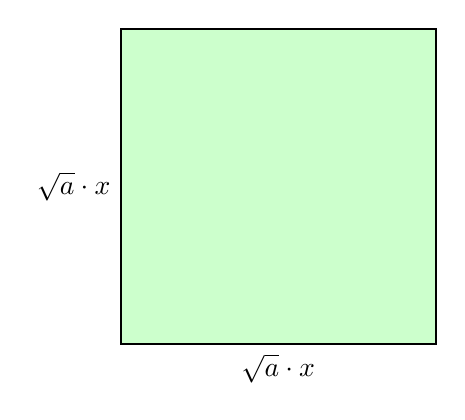
\begin{tikzpicture}[thick, scale=1]
        \fill [color=green,opacity=0.2] (0,0) rectangle +(4,4);
        \draw (0,0) rectangle +(4,4);
        \path (0,0) -- (4,0) node[midway,below] {$\sqrt{a}\cdot x$};
        \path (0,0) -- (0,4) node[midway,left] {$\sqrt{a}\cdot x$};
    \end{tikzpicture}
\end{center}

那么如何表示 $bx$ 项呢?配方本质是将原正方形扩展为更大的正方形。为此,我们在正方形周围添加矩形。将 $bx$ 代表的面积拆分为两个矩形,每个面积为 $\frac{b}{2}x$。由于矩形的一条边需与正方形边长一致(即 $\sqrt{a} \cdot x$),且面积为 $\frac{b}{2}x$,则另一条边长必为 $\frac{b}{2\sqrt{a}}$:

\begin{center}
    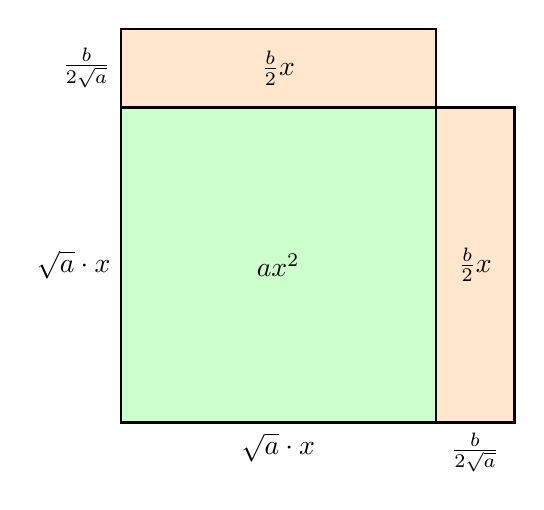
\begin{tikzpicture}[thick, scale=1]
        \fill [color=green,opacity=0.2] (0,0) rectangle +(4,4);
        \draw (0,0) rectangle +(4,4) node[pos=.5, align=center]{$ax^2$};
        \path (0,0) -- (4,0) node[midway,below] {$\sqrt{a}\cdot x$};
        \path (0,0) -- (0,4) node[midway,left] {$\sqrt{a}\cdot x$};

        \fill [color=orange,opacity=0.2] (4,0) rectangle +(1,4);
        \draw (4,0) rectangle +(1,4) node[pos=.5, align=center]{$\frac{b}{2}x$};
        \path (4,0) -- (5,0) node[midway,below] {$\frac{b}{2\sqrt{a}}$};

        \fill [color=orange,opacity=0.2] (0,4) rectangle +(4,1);
        \draw (0,4) rectangle +(4,1) node[pos=.5, align=center]{$\frac{b}{2}x$};
        \path (0,4) -- (0,5) node[midway,left] {$\frac{b}{2\sqrt{a}}$};
    \end{tikzpicture}
\end{center}

为使图形构成完整正方形,只需在右上角补上一个小正方形即可。小正方形边长为 $\frac{b}{2\sqrt{a}}$,故面积为 $\frac{b^2}{4a}$——这正是我们需要添加的项:

\begin{center}
    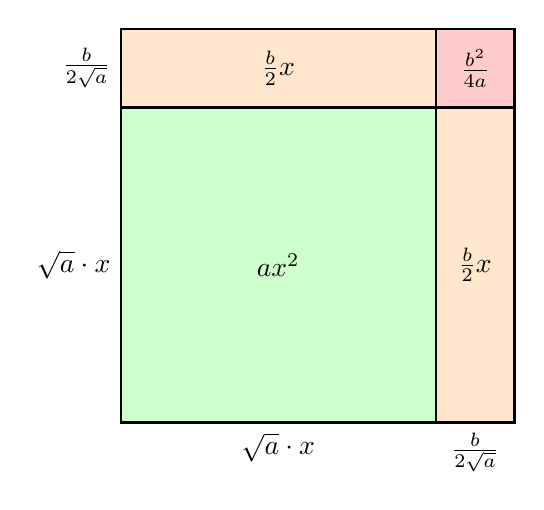
\begin{tikzpicture}[thick, scale=1]
        \fill [color=green,opacity=0.2] (0,0) rectangle +(4,4);
        \draw (0,0) rectangle +(4,4) node[pos=.5, align=center]{$ax^2$};
        \path (0,0) -- (4,0) node[midway,below] {$\sqrt{a}\cdot x$};
        \path (0,0) -- (0,4) node[midway,left] {$\sqrt{a}\cdot x$};

        \fill [color=orange,opacity=0.2] (4,0) rectangle +(1,4);
        \draw (4,0) rectangle +(1,4) node[pos=.5, align=center]{$\frac{b}{2}x$};
        \path (4,0) -- (5,0) node[midway,below] {$\frac{b}{2\sqrt{a}}$};

        \fill [color=orange,opacity=0.2] (0,4) rectangle +(4,1);
        \draw (0,4) rectangle +(4,1) node[pos=.5, align=center]{$\frac{b}{2}x$};
        \path (0,4) -- (0,5) node[midway,left] {$\frac{b}{2\sqrt{a}}$};

        \fill [color=red,opacity=0.2] (4,4) rectangle +(1,1);
        \draw (4,4) rectangle +(1,1) node[pos=.5, align=center]{$\frac{b^2}{4a}$};
    \end{tikzpicture}
\end{center}

看呐!这与代数推导的结果完全一致。添加此项后,表达式可分解为完全平方,只需再减去该项,以确保原表达式不变。

这是一个值得牢记的技巧,它能帮你理解配方的动机和步骤。但请思考:为何此方法成立?绘图时我们假设了 $a, b > 0$,那么当 $a$ 和 $b$ 为任意实数时,配方公式为何依然有效?

\subsubsection*{二次函数求根公式}

让我们回到多项式求根问题。具体来说,让我们回忆一下\textbf{二次函数求根公式}。你可能已经记住这个公式是``求解二次方程''的一种方法,但你知道它为什么成立吗?让我们试着弄清楚吧!一般来说,我们从以下形式的二次多项式开始
\[p(x) = ax^2 + bx + c\]
其中 $a \ne 0$(否则它就不是二次多项式),并且我们想要求 $p(x) = 0$ 时 $x$ 的值。(你是否尝试过回答我们上面提出的关于此类多项式有几个根的问题?在以下推导过程中请留意这一点。)将该多项式因式分解为线性因子很麻烦,所以我们使用上面介绍的方法:配方法。该方法的好处是,我们可以设 $p(x)=0$,并在配方后重新整理来求解 $x$。
\[0 = p(x) = ax^2 + bx + c =a\Big(x+\frac{b}{2a}\Big)^2+\Big(c- \frac{b^2}{4a}\Big)\]
化简可得
\[\frac{b^2}{4a} -c = a\Big(x+\frac{b}{2a}\Big)^2\]

现在,我们要开始``撤消''此处的配方来求解 $x$,这需要对两边求平方根。但如果 $\frac{b^2}{4a} -c < 0$ 呢?我们根本无法求平方根!如果 $\frac{b^2}{4a} -c = 0$ 呢?会有什么问题吗?当 $\frac{b^2}{4a} -c > 0$ 时会有什么问题吗?这些问题与多项式根的个数相关。你可能已经(正确地)推断出二次多项式最多可以有两个根,但在这里我们发现二次多项式可能有一个或零个根(及其原因)!

\begin{itemize}
    \item 当 $\frac{b^2}{4a} -c < 0$ 时,那么 $x$ 的任何值都\emph{不}可能满足上面推导中的最后一行公式。因此,$p(x)$ 无实数根。
    \item 当 $\frac{b^2}{4a} -c = 0$ 时,那么对上面最后一行公式两边取平方根是完全有效的,但只会产生\emph{唯一一个} $x$ 值:
    \begin{align*}
        \frac{b^2}{4a} -c = 0 &= a\Big(x+\frac{b}{2a}\Big)^2 \\
        0 &= x+\frac{b}{2a} \\
        x &= -\frac{b}{2a}
    \end{align*}
    \item 当 $\frac{b^2}{4a} -c > 0$ 时,此时 $p(x)$ 有\emph{两个}根,因为两边取平方根会引入两个可能的解。一般来说,当我们遇到像 $s^2 = t$ 这种情况时,可能的解是 $s =\sqrt{t}$ 和 $s = -\sqrt{t}$,但我们必须同时考虑两者(通常将其写做 $s = \pm\sqrt{t}$)。在这种情况下求解 $x$ 得
    \begin{align*}
        \frac{b^2}{4a} -c &= a\Big(x+\frac{b}{2a}\Big)^2 \\
        \pm\sqrt{\frac{b^2-4ac}{4a}} &= \sqrt{a}\Big(x+\frac{b}{2a}\Big) = \sqrt{a}x+\frac{b}{2\sqrt{a}} \\
        -\frac{b}{2\sqrt{a}}\pm\frac{\sqrt{b^2-4ac}}{\sqrt{4a}} &= \sqrt{a}x \\
        -\frac{b}{2a}\pm\frac{\sqrt{b^2-4ac}}{\sqrt{4a^2}} &= x
    \end{align*}
    现在,我们必须谨慎对待取平方根。一般来说,$\sqrt{4a^2} = \pm2a$,但分子上的平方根项已经有了一个 $\pm1$ 因子,分母上的因子不会改变这一点。因此,我们可以得出结论
    \[x = -\frac{b}{2a}\pm\frac{\sqrt{b^2-4ac}}{2a} = \frac{-b\pm\sqrt{b^2-4ac}}{2a}\]
    这就是二次函数求根公式!
\end{itemize}

请记住,推导的最后一种情况是在 $\frac{b^2}{4a} -c > 0$ 的假设下进行的。当 $\frac{b^2}{4a} -c = 0$ 时,该公式依然适用吗?在这种假设下,我们是否可以执行与上面相同的步骤?为什么可以或者为什么不行?

\subsubsection*{习题}

\begin{problem}
    求满足 $x-a$ 整除 $x^2+2ax-3$ 的 $a$ 的所有可能值。
\end{problem}
\begin{problem}
    求使得 $x^3 + b$ 可以被 $x + b$ 整除的 $b$ 的所有可能值。
\end{problem}
\begin{problem}
    对于任意自然数 $n$,将 $x^n - 1$ 因式分解。
\end{problem}
\begin{problem}
    求由如下公式定义的 $x$ 的值
    \[x = \sqrt{2+\sqrt{2+\sqrt{2+\sqrt{2+\dots}}}}\]
    \begin{hint}
        尝试用 $x$ 本身来表示无限嵌套根式。
    \end{hint}
\end{problem}
\begin{problem}
    用配方法证明:任意正数 $n$ 及其倒数之和始终大于或等于 $2$,并且唯一使和等于 $2$ 的数字是 $n = 1$。
    \begin{hint}
        求和,加减 $2$,然后重新整理。
    \end{hint}
\end{problem}
\begin{problem}
    如何求解形如 $ax^4 + bx^2 + c$ 的四次多项式的根?
\end{problem}
